\documentclass[12pt,letterpaper]{article}
\usepackage{graphicx,textcomp}
\usepackage{natbib}
\usepackage{setspace}
\usepackage{fullpage}
\usepackage{color}
\usepackage[reqno]{amsmath}
\usepackage{amsthm}
\usepackage{fancyvrb}
\usepackage{amssymb,enumerate}
\usepackage[all]{xy}
\usepackage{endnotes}
\usepackage{adjustbox}
\usepackage{lscape}
\newtheorem{com}{Comment}
\usepackage{float}
\usepackage{hyperref}
\newtheorem{lem} {Lemma}
\newtheorem{prop}{Proposition}
\newtheorem{thm}{Theorem}
\newtheorem{defn}{Definition}
\newtheorem{cor}{Corollary}
\usepackage{enumitem}

\newtheorem{obs}{Observation}
\usepackage[compact]{titlesec}
\usepackage{dcolumn}
\usepackage{tikz}
\usetikzlibrary{arrows}
\usepackage{multirow}
\usepackage{xcolor}
\newcolumntype{.}{D{.}{.}{-1}}
\newcolumntype{d}[1]{D{.}{.}{#1}}
\definecolor{light-gray}{gray}{0.65}
\usepackage{url}
\usepackage{listings}
\usepackage{color}

\definecolor{codegreen}{rgb}{0,0.6,0}
\definecolor{codegray}{rgb}{0.5,0.5,0.5}
\definecolor{codepurple}{rgb}{0.58,0,0.82}
\definecolor{backcolour}{rgb}{0.95,0.95,0.92}

\lstdefinestyle{mystyle}{
	backgroundcolor=\color{backcolour},   
	commentstyle=\color{codegreen},
	keywordstyle=\color{magenta},
	numberstyle=\tiny\color{codegray},
	stringstyle=\color{codepurple},
	basicstyle=\footnotesize,
	breakatwhitespace=false,         
	breaklines=true,                 
	captionpos=b,                    
	keepspaces=true,                 
	numbers=left,                    
	numbersep=5pt,                  
	showspaces=false,                
	showstringspaces=false,
	showtabs=false,                  
	tabsize=2
}
\lstset{style=mystyle}
\newcommand{\Sref}[1]{Section~\ref{#1}}
\newtheorem{hyp}{Hypothesis}

\title{Answer Key: Problem Set 4}
\date{Jeffrey Ziegler}
\author{Applied Stats II}

\begin{document}
	\maketitle
	
	\section*{Instructions}
	\begin{itemize}
		\item \textit{Please show your work! You may lose points by simply writing in the answer. If the problem requires you to execute commands in \texttt{R}, please include the code you used to get your answers. Please also include the \texttt{.R} file that contains your code. If you are not sure if work needs to be shown for a particular problem, please ask.}
			\item \textit{Your homework should be submitted electronically on GitHub in \texttt{.pdf} form.}
			\item \textit{This problem set is due before 23:59 on Wednesday April 12, 2024. No late assignments will be accepted.}
	\end{itemize}
	\vspace{.25cm}
	
	\section*{Question 1}
	\vspace{.25cm}
	\noindent \emph{We're interested in modeling the historical causes of child mortality. We have data from 26855 children born in Skellefteå, Sweden from 1850 to 1884. Using the "child" dataset in the \texttt{eha} library, fit a Cox Proportional Hazard model using mother's age and infant's gender as covariates. Present and interpret the output.}\\
	
	First, let's estimate our Cox proportional hazard model:
	\vspace{.25cm}
	\lstinputlisting[language=R, firstline=39,lastline=43]{../answer_key/PS4_answerKey.R} 
	\vspace{.25cm}
	\noindent Looking at Table~\ref{table:coefficients}, we can interpret the estimated coefficient for gender as the logged hazard ratio of boys with respect to girls for infants with mothers of the same age. If we exponentiate the estimated coefficient of gender (exp(coef)= 0.923), we see that girls are about 8\% more likely to survive than girls with mothers of the same age (HR $< 1$ = reduction in the hazard). Looking at the age coefficient, we can see that having an older mother (holding infant gender constant) is also a “poor prognostic factor” that increases the risk of death. More specifically, a one unit increase in mother's age is associated with an increase in the logged hazard ratio for infants of the same gender.
	
		\begin{table}[h!]
		\caption{\footnotesize Cox Proportional Hazard model results}
		\vspace{.25cm}
		\label{table:coefficients}
		\centering
		\begin{adjustbox}{width=.3\textwidth}
			\begin{tabular}{l c}
				\hline
			m.age       & $0.01^{***}$ \\
            & $(0.00)$     \\
sex\_female   & $-0.08^{**}$ \\
            & $(0.03)$     \\
\hline
AIC         & $113010.97$ \\
\# events & $5616$     \\
N   & $26574$    \\

				\hline
				\multicolumn{2}{l}{\footnotesize{$^{***}p<0.001$; $^{**}p<0.01$; $^{*}p<0.05$}}
			\end{tabular}
		\end{adjustbox}
	\end{table}
	
%	To visually investigate the relationship between gender and mothers’ age further, we can see that in Figure 1, children generally survive longer when they have older mothers (which may be symptomatic of access to healthcare and economic class). Moreover, we can see that boys generally survive longer than girls (most likely due to selective gender preferences of children in the 19th century).
%	
%		
%	\begin{figure}[h!]\centering
%		\caption{\footnotesize Predicted hazard ratio by gender and mother age.}%\vspace{-1cm}
%		\label{fig:coxph}
%				\vspace{.25cm}
%		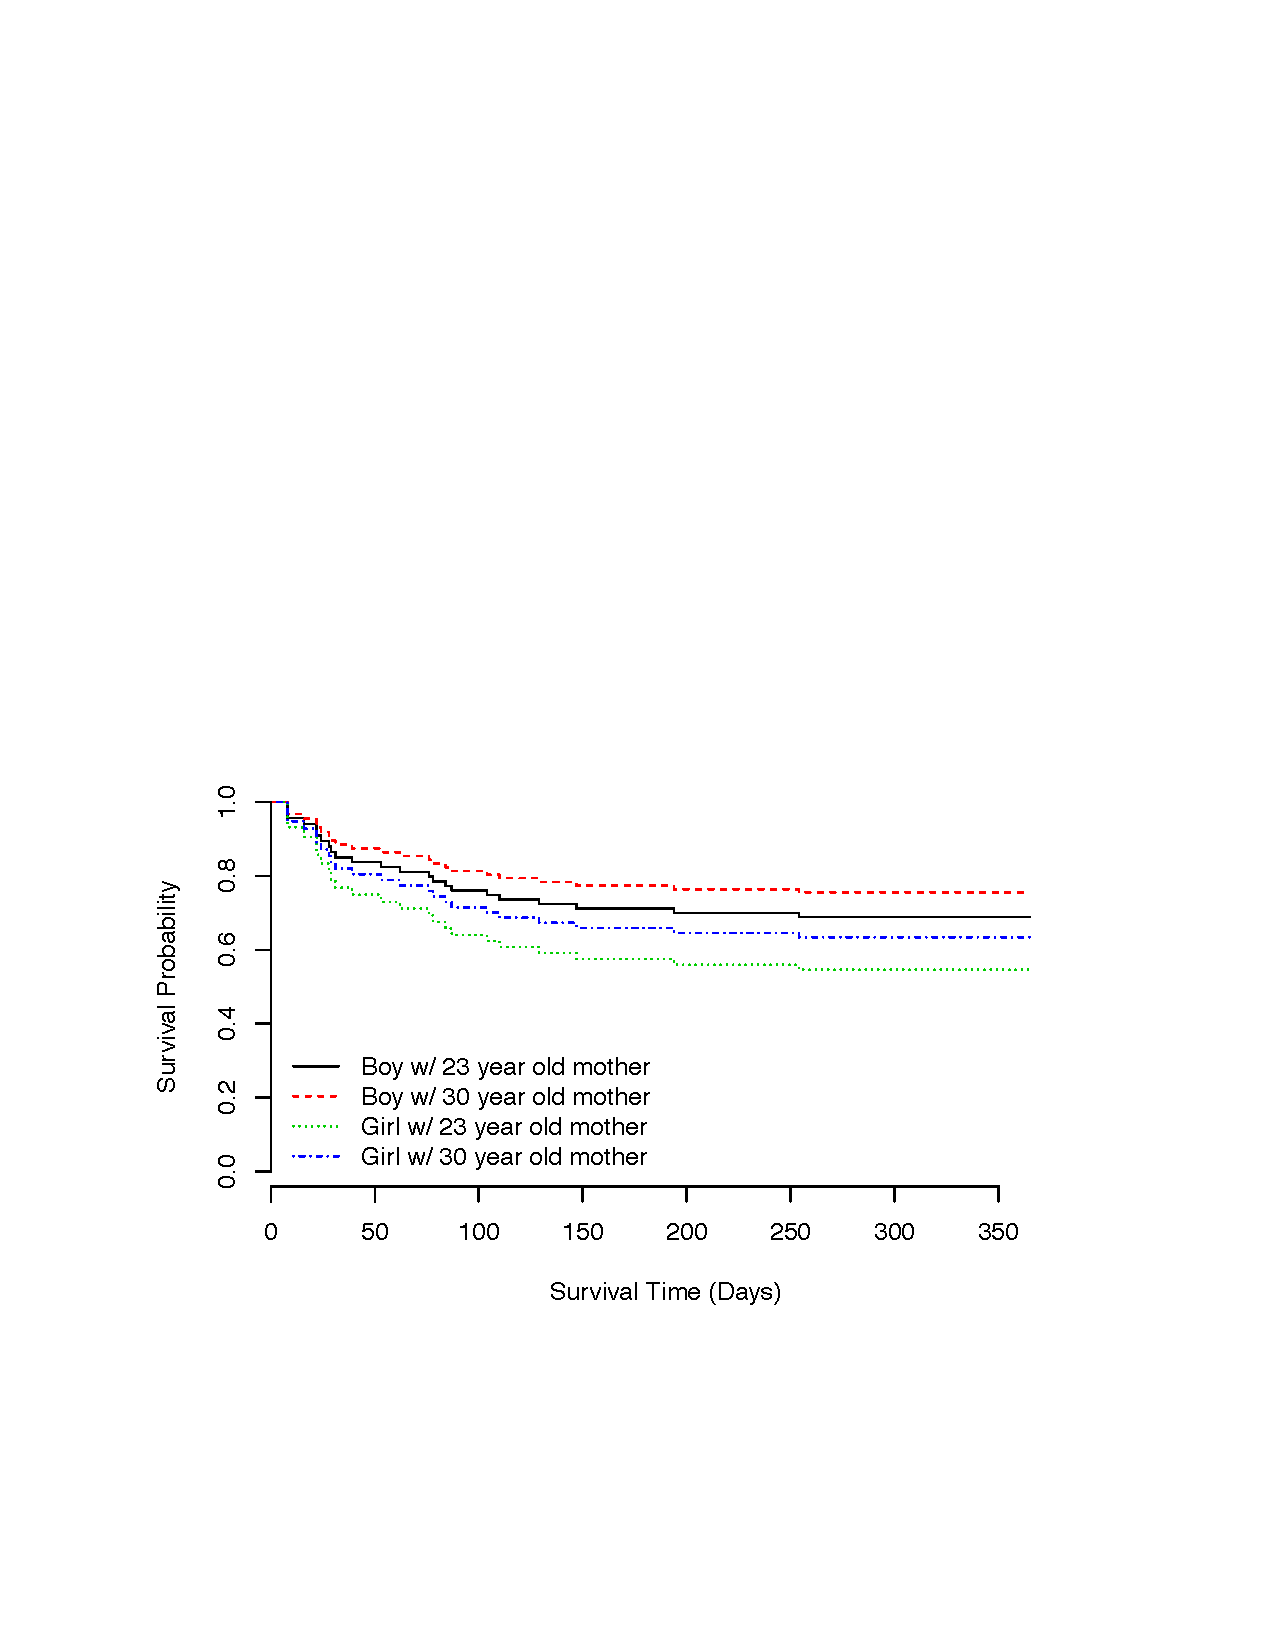
\includegraphics[width=.99\textwidth]{../../../../graphics/ps4_fig1.pdf}\\
%	\end{figure}


\end{document}
